\chapter{The impact of HIFI standing waves on the determination of the physical parameters of the star-forming region S140}
\chaptermark{Standing waves on S140}
\label{sec:chapter5}
\section{Introduction}

In this chapter, we examine how the estimation of astrophysical parameters is affected by standing waves in the instrument.
We attempt to derive the kinetic temperature of a molecular cloud from \ce{CO} line ratios.

With the Heterodyne Instrument for the Far Infrared (HIFI) of the Herschel Space Observatory,
we measured spectra of the \transition{CO}{8}{7} and \transition{CO}{9}{8} transition lines of the source S140 IRS1.
Each transition was measured with different optical settings in order to modulate standing waves.

We used the Radex software by van der Tak et al.\ \cite{vandertak2007radex} to recover kinetic temperatures from the measured line ratios.
The variations of the line ratios translate into uncertainties on the temperature.
We illustrate that standing waves can have a dramatic impact on the estimation of physical parameters.

\subsection{S140 IRS1}
S140 is a high-mass star-forming region of the molecular cloud L1204.
At its core resides the very bright ($L \geqslant 10^5 L_{\odot}$ \cite{demuizon1980}), therefore massive, young stellar object IRS1.
IRS1 is located inside S140 at $\alpha = 22^\text{h} 19^\text{m} 18.21^\text{s}$ $\delta = \ang{63;18;46.9}$ (J2000) in the Cepheus constellation, \SI{910}{pc} away.
As shown on \cref{fig:12CO10_moment0}, IRS1 is one of three notable infrared sources in S140 \cite{maud2013s140}.

The south-western part of S140 is ionized by the ultraviolet radiation of the B0V star HD~211880.
The resulting ionization front is marked ``IF'' on \cref{fig:12CO10_moment0}.
It corresponds to a \ce{H+} photon-dominated region.
However, IRS1 is located in a much cooler and denser environment relatively unaffected by HD~211880.
Therefore, evidence of high temperatures around IRS1 should be attributed to the young stellar objects themselves.
\begin{figure}[hbtp]
    \centering
    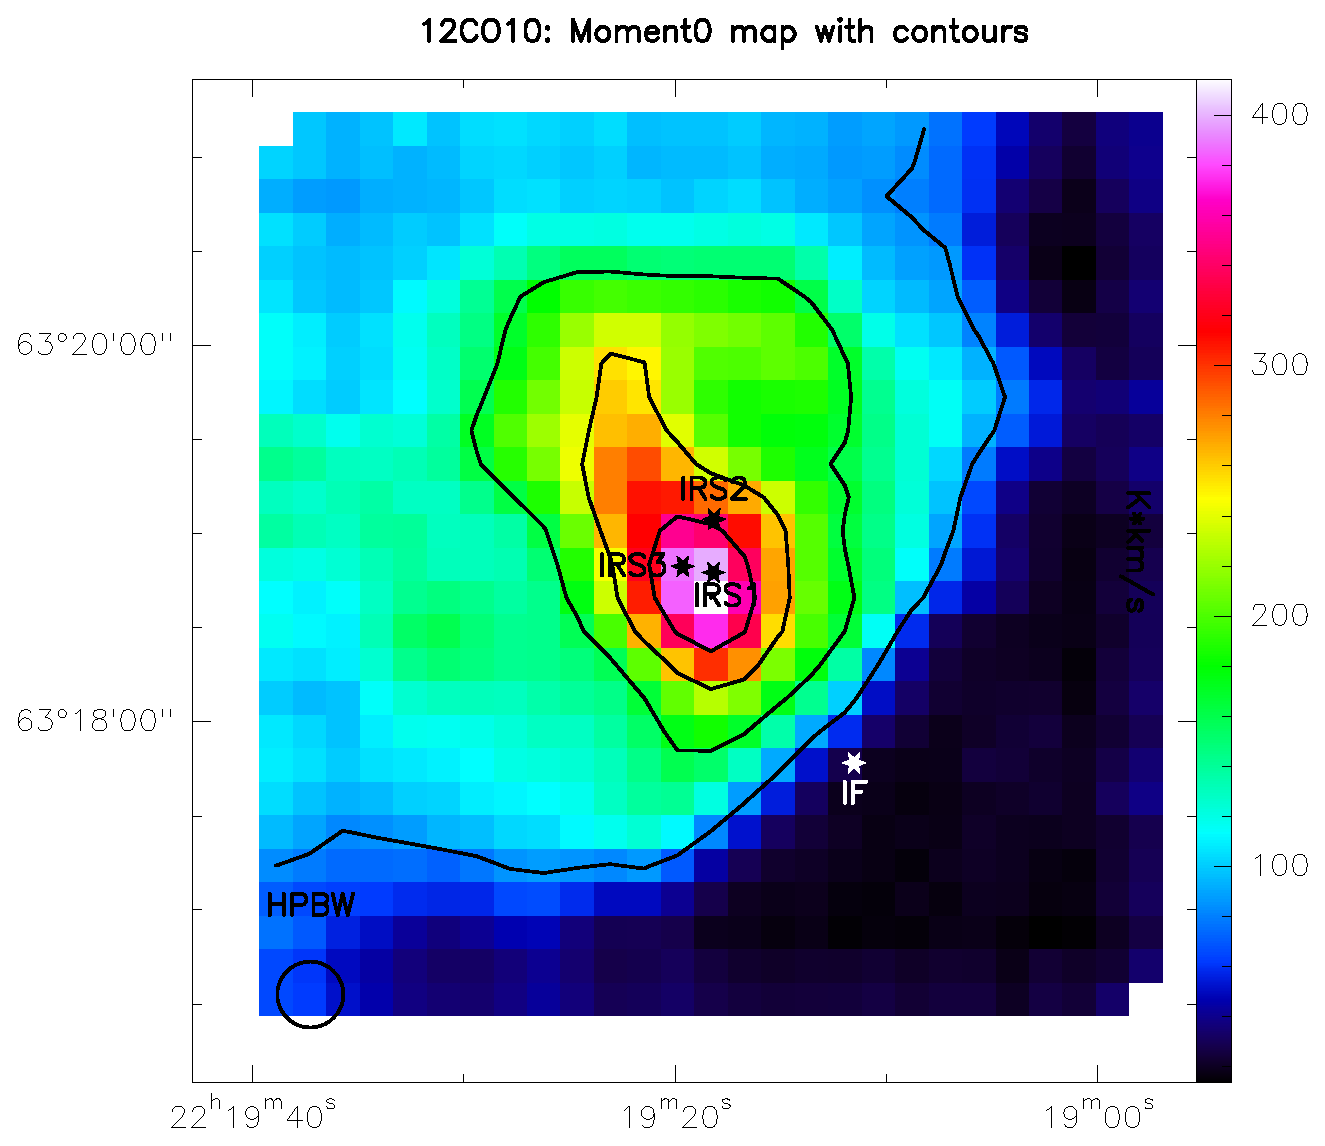
\includegraphics[width=\textwidth]{12CO10_moment0}
    \caption{Map of \transition{CO}{1}{0} around S140 IRS1, taken by the \SI{30}{\meter} telescope of IRAM. Credit E. Koumpia.}
    \caption*{
        The color scale represents the integrated intensity in \si{\kelvin \kilo\meter \per \second}.
        The beam width (HPBW) is represented by the circle in the bottom left.
        The beam width of the \SI{30}{\meter} telescope at the frequency of the \transition{CO}{1}{0} transition is \SI{21}{\arcsec}.
        Coincidentally, \SI{21}{\arcsec} is also the beam width of the Herschel Space Observatory at the frequency of the \transition{CO}{9}{8} transition.
    }
    \label{fig:12CO10_moment0}
\end{figure}

\subsection{CO}
Dense molecular clouds such as star-forming regions contain mostly molecular hydrogen \ce{H2} and dust.
Dust is opaque to optical and near-infrared radiation but is transparent in the submillimetric domain, which makes submillimetric spectroscopy a tool of choice to study star formation.
Unfortunately, the rotational lines of \ce{H2} are in the mid-infrared range and occur at temperatures above~\SI{500}{\kelvin}, making \ce{H2} invisible in cold molecular clouds.
However, other less abundant species can interact with \ce{H2} in a measurable way.
This is the case for carbon monoxide \ce{CO} which emits rotational lines when it collides with \ce{H2}, see \cref{table:co_transition_frequencies}.
Because \ce{CO} is relatively abundant and stable in molecular clouds, it is considered a tracer of \ce{H2}.

\begin{table}[hbtp]
    \centering
    \begin{tabular}{lSS} % S is from SIunitx.
        \toprule
        transition &
        % Use multicolumn to protect the header from the influence of S.
        \multicolumn{1}{c}{rest frequency [\si{\giga\hertz}]} &
        \multicolumn{1}{c}{excitation temperature [\si{\kelvin}]} \\
        \midrule
        \transition{CO}{5}{4}   &  576.2679305 &  82.97 \\
        \transition{CO}{6}{5}   &  691.4730763 & 116.16 \\
        \transition{CO}{7}{6}   &  806.6518060 & 154.87 \\
        \transition{CO}{8}{7}   &  921.7997000 & 199.11 \\
        \transition{CO}{9}{8}   & 1036.9123930 & 248.88 \\
        \transition{CO}{10}{9}  & 1151.9854520 & 304.16 \\
        \transition{CO}{11}{10} & 1267.0144860 & 364.97 \\
        \transition{CO}{12}{11} & 1381.9951050 & 431.29 \\
        \transition{CO}{13}{12} & 1496.9229090 & 503.13 \\
        \transition{CO}{14}{13} & 1611.7935180 & 580.49 \\
        \transition{CO}{15}{14} & 1726.6025057 & 663.35 \\
        \transition{CO}{16}{15} & 1841.3455060 & 751.72 \\
        \bottomrule
    \end{tabular}
    \caption{
        Rest frequencies and excitation temperature of
        the collisional rotation lines of \ce{CO} detectable by HIFI.
        Credit: Leiden Atomic and Molecular Database \cite{schoier2004leidenmoldb}.
    }
    \label{table:co_transition_frequencies}
\end{table}


\subsection{HIFI}

The Heterodyne Instrument for the Far Infrared operates between \SI{480}{\giga\hertz} and \SI{1910}{\giga\hertz}, that is between \SI{625}{\micro\meter} and \SI{157}{\micro\meter}.
Its heterodyne design allows it to produce spectra with a resolution $\Delta f/ f$ between \num{6.5e-8} and \num{2.3e-6}.

In a heterodyne instrument, a mixer combines the signal from the sky with the signal from a monochromatic phase-locked source called ``local oscillator'' (LO).
The non-linearity of the mixer allows it to change the frequency of the incoming signals.
The signal produced by the mixer at a frequency $f_\text{i}$ is related to the incoming signals at $f_\text{LO}-f_\text{i}$ and $f_\text{LO}+f_\text{i}$.
These are the two sky frequencies that are observed for a given $f_\text{LO}$ and $f_\text{i}$.
In HIFI, $f_\text{i} \in [\SI{4}{\giga\hertz}, \SI{8}{\giga\hertz}]$, a range of frequency for which we can build high-resolution spectrometers.

HIFI has two backends.
The signal delivered by the mixer can be directed toward the WideBand Spectrometer (WBS) or the High Resolution Spectrometer (HRS).
In this chapter, we study spectra aquired with the WBS.
Information about the HRS, and HIFI in general, can be found in the paper by \citeauthor{AA_518_L6} \cite{AA_518_L6}.

The WBS is an acousto-optic spectrometer.
Its resolution is fixed at \SI{1.1}{\mega\hertz} and its instantaneous bandwidth covers the whole range of 4 to \SI{8}{\giga\hertz} of the mixer.

No single mixer \todo{at least today, or maybe we can but with a horrible S/N ratio?} can cover the whole HIFI range of \SIrange{480}{1910}{\giga\hertz}.
HIFI uses seven mixer bands to cover that range.
Five bands use SIS mixers, two use HEB mixers.
Each mixer band also needs two LO subbands.
In addition to having its own mixer and LO, each band requires its own optics, its own way of injecting the LO power into the sky signal, its own way of focusing the signals onto the mixers.
This makes HIFI a very complex device which can be seen as $7 \times 2 =14$ independant instruments.
Finally, each mixer band has two mixers: one for each polarization.

\todo[inline]{Picture of the FPU to illustrate that wall of text.}







\section{Observation}

We scheduled two observations of S140 IRS1 with HIFI.
They are available in the Herschel Science Archive and can be retrieved with the following observation identifiers (``obsid''):
\begin{itemize}
    \item obsid 0x50015e1d, band 3b, \transition{CO}{8}{7},
    \item obsid 0x50015d89, band 4a, \transition{CO}{9}{8}.
\end{itemize}

These observations use a non-standard observing mode based on the standard dual beam switch spectral scan.
The non-standard aspect of this observing mode is that, for each local oscillator frequency, there are 19 diplexer settings instead of 1.
This means that we willingly mistune the diplexer around its optimal position.
\Cref{tab:lo_frequencies} gives the five LO frequencies used for each transition
and \cref{tab:diplexer_currents} gives the nineteen diplexer settings used for each LO frequency and each transition.
\begin{table}[hbtp]
    \centering
    \begin{tabular}{cSSSSS}
        \toprule
        transition & \multicolumn{5}{c}{LO frequencies [\si{\giga\hertz}]} \\
        \midrule
\transition{CO}{8}{7} &  914.4045 &  914.4225 &  914.4450 &  914.4630 &  914.4810 \\
\transition{CO}{9}{8} & 1029.4830 & 1029.5010 & 1029.5190 & 1029.5415 & 1029.5595 \\
        \bottomrule
    \end{tabular}
    \caption{
        Frequencies at which the local oscillator was tuned.
    }
    \label{tab:lo_frequencies}
\end{table}
\begin{table}[hbtp]
    \centering
    \begin{tabular}{cSSSSS}
        \toprule
        transition & \multicolumn{5}{c}{diplexer actuator currents [\si{\milli\ampere}]} \\
        \midrule
        \multirow{4}{*}{\transition{CO}{8}{7}}
        & 0.503 & 0.499 & 0.493 & 0.488 & 0.481 \\
        & 0.476 & 0.471 & 0.465 & 0.458 & 0.453 \\
        & 0.447 & 0.442 & 0.435 & 0.430 & 0.425 \\
        & 0.419 & 0.412 & 0.407 & 0.401 & \\
        \midrule
        \multirow{4}{*}{\transition{CO}{9}{8}}
        & 1.336 & 1.332 & 1.325 & 1.318 & 1.313 \\
        & 1.306 & 1.300 & 1.293 & 1.288 & 1.281 \\
        & 1.275 & 1.269 & 1.263 & 1.256 & 1.251 \\
        & 1.244 & 1.237 & 1.232 & 1.225 & \\
        \bottomrule
    \end{tabular}
    \caption{
        Currents applied to the actuator of the H diplexer for each LO frequency.
    }
    \label{tab:diplexer_currents}
\end{table}

A hot-cold measurement is made before each measurement on the sky.


Because the observing mode is not standard, the default data reduction pipeline does not process the data adequately.
It is necessary to rerun the pipeline from the level 0 to the level 2 with a custom configuration.
The ``doAverage'' task of the pipeline must be disabled (otherwise all the spectra with different diplexer settings are averaged together which is not what we want).
Another reason to rerun the pipeline is a bug in the frequency calibration affecting these observations only; it is necessary to use the pipeline of HIPE version 13, or at least a late build of HIPE 12 (2518 or later) in which that bug is corrected.

A dual beam switch observing mode was chosen to remove the baseline due to extended emission.  The OFF position is \SI{3}{\arcmin}

On position
$\alpha = 22^\text{h} 19^\text{m} 18.21^\text{s}$ $\delta = \ang{63;18;46.9}$ (J2000)

Off position, three minutes North West away from the On.
$\alpha = 22^\text{h} 19^\text{m} 11^\text{s}$ $\delta = \ang{63;21;40}$ (J2000)
It is trying to avoid the IF and the star.
It's not the emptiest position ever but at least on the \transition{CO}{1}{0} map, it looks vaguely empty.
Still trying to look at an OFF spectrum to see if there's a line, but the HSA just died on me.


It is probable that there is some CO emission in the OFF.  If so, then our lines appear lower than they should.

Each transition is observed at 5 local oscillator frequencies, and for each of these at 19 diplexer tunings.
This gives $5 \times 19 = 95$ spectra per transition for a total of 190 spectra.

%The local oscillator frequencies chosen are
%\num{914.4045}, \num{914.4225}, \num{914.4450}, \num{914.4630} and \SI{914.4810}{\giga\hertz}
%\num{1029.4830}, \num{1029.5010}, \num{1029.5190}, \num{1029.5415} and \SI{1029.5595}{\giga\hertz}.

%This should allow us to measure which of the two effects dominates.  There may also be enough information to derive the reflection coefficients of the LO and the mixer, at least for these 5 frequencies.  Do these coefficients jump a lot or do they vary smoothly?

\section{Results}

We focused on the data measured by the horizontally polarized wideband spectrometer of HIFI.
Indeed, the vertical polarization suffers from frequency calibration issues and is therefore less reliable.

\Cref{fig:co98_full_bandwidth} presents one of the 190 spectra acquired during this observation.
The \ce{CO} line is always relatively narrow compared to the instantaneous bandwidth of the instrument, and in the rest of this chapter we will often zoom in on the line.
Furthermore, the line is always placed on the high-frequency end of that bandwidth, never in the center, which exposes the line to a higher number of standing waves due to the nature of the diplexer. \todo{refer to a sideband simulation of chapter 3}
\begin{figure}[hbtp]
    \centering
    \includegraphics{50015d89_WBS-H-USB_00-00_full}
    \caption{
        One spectrum of \transition{CO}{9}{8} shown with its full \SI{4}{\giga\hertz} bandwidth.
    }
    \label{fig:co98_full_bandwidth}
\end{figure}

\Cref{fig:overview_co87} and \cref{fig:overview_co98} show all the spectra measured for \transition{CO}{8}{7} and \transition{CO}{9}{8} respectively.
For each LO frequency, 19 spectra are measured with different settings of the diplexer actuator current.
For each transition, the 95 spectra are stacked in a color plot, sorted either by LO frequency then diplexer setting, or by diplexer setting then LO frequency.

\begin{figure}
    \centering
    \includegraphics[width=.9\textwidth]{overview_co87}
    \includegraphics[width=.9\textwidth]{overview_co87_flipped}
    \caption{The 95 spectra of \transition{CO}{8}{7}, 5 LO frequencies times 19 diplexer settings.
    Top: sorted by LO then diplexer.  Bottom: sorted by diplexer then LO.}
    \label{fig:overview_co87}
\end{figure}
\begin{figure}
    \centering
    \includegraphics[width=.9\textwidth]{overview_co98}
    \includegraphics[width=.9\textwidth]{overview_co98_flipped}
    \caption{The 95 spectra of \transition{CO}{9}{8}, 5 LO frequencies times 19 diplexer settings.
    Top: sorted by LO then diplexer.  Bottom: sorted by diplexer then LO.}
    \label{fig:overview_co98}
\end{figure}





\section{Analysis}
\subsection{Model}
\subsubsection{Components}
Superimposed on the spectra of \cref{fig:spectra_transitions} are the various components of a model.
The model is constituted of three or four elements:
\begin{itemize}
    \item a constant horizontal baseline,
    \item a narrow gaussian for the core emission,
    \item a broad gaussian for the outflow emission,
    \item and optionally a third negative gaussian for a self-absorption component.
\end{itemize}
Both transitions show a self absorption, but in the case \transition{CO}{9}{8}, the self-absorption barely sticks out of the noise which makes it too difficult to fit.
The baseline is not represented on \cref{fig:spectra_transitions}, it is silently added to each gaussian model on the plots.

\begin{figure}[hbtp]
    \centering
    \begin{subfigure}[b]{\textwidth}
        \includegraphics{50015e1d_WBS-H-USB_00-00}
        \caption{\transition{CO}{8}{7}}
    \end{subfigure}
    \\
    \begin{subfigure}[b]{\textwidth}
        \includegraphics{50015d89_WBS-H-USB_00-00}
        \caption{\transition{CO}{9}{8}}
    \end{subfigure}
    \caption{
        HIFI WBS-H spectra of S140 IRS1 for \transition{CO}{8}{7} and \transition{CO}{9}{8}.
        For each transition, the the top plot shows the data in black and the fitted model in color, where the full model is the sum of the others; and the botton plot shows the difference between the data and the full model.
        ``LO'' stands for ``local oscillator frequency'' and ``DAC'' for ``diplexer attenuator current''.
    }
    \label{fig:spectra_transitions}
\end{figure}

To convert the frequencies $f$ into velocities $v$, we used the Doppler formula \eqref{eq:doppler} in which $c$ denotes the speed of light.
We applied it with the rest frequencies
$f_0 = \SI{ 921.7997000}{\giga\hertz}$ and
$f_0 = \SI{1036.9123930}{\giga\hertz}$
for \transition{CO}{8}{7} and \transition{CO}{9}{8} respectively.
These values are taken from \cref{table:co_transition_frequencies} and come from the Leiden Atomic and Molecular Database \cite{schoier2004leidenmoldb}.

\begin{equation}
    v = c \left( \frac{f_0}{f} - 1 \right) \label{eq:doppler}
\end{equation}

The model for the baseline is a constant $B$.
The model for a gaussian takes three parameters:
an amplitude $a$,
a position $b$ and
a standard deviation $c$
according to \cref{eq:gaussian}.
\begin{equation}
    f(a, b, c, x) = a \mathrm{e}^{- \frac{(x - b)^2}{2 c^2}} \label{eq:gaussian}
\end{equation}

The model used for \transition{CO}{8}{7}, which uses one baseline and three gaussians, is given by \cref{eq:model_co87}.
The model for \transition{CO}{9}{8}, with two gaussians only, is given by \cref{eq:model_co98}.

\begin{align}
    m_{87}(x) &= B + f(a_0, b_0, c_0, x) + f(a_1, b_1, c_1, x) + f(a_2, b_2, c_2, x)
    \label{eq:model_co87}
    \\
    m_{98}(x) &= B + f(a_0, b_0, c_0, x) + f(a_1, b_1, c_1, x)
    \label{eq:model_co98}
\end{align}


\subsubsection{Sideband ratio}
In our observations, we willigly mistuned the diplexer.
We did it in order to explore the effect of the diplexer on the standing waves.
Unfortunately, detuning the diplexer also has a first-order effect on our spectra, even without standing waves, that we must correct before continuing our analysis.




\begin{figure}
        \centering
    \begin{subfigure}[b]{\textwidth}
        \includegraphics{diplexer_correction_no}
        \caption{Before compensating for the sideband ratio imbalance due to the diplexer.}
    \end{subfigure}
    \\
    \begin{subfigure}[b]{\textwidth}
        \includegraphics{diplexer_correction_yes}
        \caption{After compensating for the sideband ratio imbalance due to the diplexer.}
    \end{subfigure}
\end{figure}

\subsubsection{Fit results}
We fitted the parameters $B$, $a_0$, $b_0$, $c_0$, $a_1$, $b_1$, $c_1$, and optionally $a_2$, $b_2$ and $c_2$, for each spectrum independantly, with a least-square Levenberg-Marquardt algorithm.

\Crefrange{fig:fit_base}{fig:fit_sabs} present the fitted parameters.
The horizontal axis of each plot corresponds to the spectrum number.
There are 95 spectra for each transition, therefore 95 points on each plot.
The spectra are ordered by LO frequecy first, then by diplexer setting, which is similar to the upper plots of figures~\ref{fig:overview_co87} and~\ref{fig:overview_co98}.
These plots show the model parameters for \transition{CO}{8}{7} on the left, and \transition{CO}{9}{8} on the right.
For the gaussian components, we plot the full width at half maximum (FWHM) instead of the standard deviation $\sigma$, for its interpretation as a line width is more visual and intuitive; both quantities are linked by~\cref{eq:fwhm_sigma}.
\begin{equation}
    \text{FWHM} = 2 \sigma \sqrt{2 \ln(2)}    \label{eq:fwhm_sigma}
\end{equation}

The fitting algorithm does not only return the optimum, it also returns an approximation of the covariance matrix at the optimum.
This allows us to add error bars to our plots.
To compute the error bars, we multiplied the diagonal of the covariance matrix by a noise scale.
In out case, the covariance matrix  is mostly dominated by its diagonal, although the velocities of the core and the outflow components are relatively strongly correlated: their covariance is only slightly lower than their individual variances.
The noise scale was obtained by computing the standard deviation of the residuals (data - model) for the 6000 first channels, which correspond to the first three quarters of each spectra.
As illustrated in~\cref{fig:co98_full_bandwidth}, the first three quarters of our spectra contains no visible molecular line, only background noise.
\todo{Give the valueS of the noise factor, like 3K or so}

\begin{figure}[hbtp]
    \centering
    \begin{subfigure}[b]{0.5\textwidth}
        \includegraphics{co87_base_inte}
        \caption{\transition{CO}{8}{7}}
    \end{subfigure}%
    \begin{subfigure}[b]{0.5\textwidth}
        \includegraphics{co98_base_inte}
        \caption{\transition{CO}{9}{8}}
    \end{subfigure}%
    \caption{
        Model of the baseline component.
    }
    \label{fig:fit_base}
\end{figure}

\begin{figure}[hbtp]
    \centering
    \begin{subfigure}[b]{0.5\textwidth}
        \includegraphics{co87_core_velo}
        \caption{\transition{CO}{8}{7} LSR velocity}
    \end{subfigure}%
    \begin{subfigure}[b]{0.5\textwidth}
        \includegraphics{co98_core_velo}
        \caption{\transition{CO}{9}{8} LSR velocity}
    \end{subfigure}%
    \\
    \begin{subfigure}[b]{0.5\textwidth}
        \includegraphics{co87_core_vfwh}
        \caption{\transition{CO}{8}{7} FWHM}
    \end{subfigure}%
    \begin{subfigure}[b]{0.5\textwidth}
        \includegraphics{co98_core_vfwh}
        \caption{\transition{CO}{9}{8} FWHM}
    \end{subfigure}%
    \\
    \begin{subfigure}[b]{0.5\textwidth}
        \includegraphics{co87_core_ampl}
        \caption{\transition{CO}{8}{7} amplitude}
    \end{subfigure}%
    \begin{subfigure}[b]{0.5\textwidth}
        \includegraphics{co98_core_ampl}
        \caption{\transition{CO}{9}{8} amplitude}
    \end{subfigure}%
    \caption{
        Gaussian model of the core component.
    }
    \label{fig:fit_core}
\end{figure}

\begin{figure}[hbtp]
    \centering
    \begin{subfigure}[b]{0.5\textwidth}
        \includegraphics{co87_outf_velo}
        \caption{\transition{CO}{8}{7} LSR velocity}
    \end{subfigure}%
    \begin{subfigure}[b]{0.5\textwidth}
        \includegraphics{co98_outf_velo}
        \caption{\transition{CO}{9}{8} LSR velocity}
    \end{subfigure}%
    \\
    \begin{subfigure}[b]{0.5\textwidth}
        \includegraphics{co87_outf_vfwh}
        \caption{\transition{CO}{8}{7} FWHM}
    \end{subfigure}%
    \begin{subfigure}[b]{0.5\textwidth}
        \includegraphics{co98_outf_vfwh}
        \caption{\transition{CO}{9}{8} FWHM}
    \end{subfigure}%
    \\
    \begin{subfigure}[b]{0.5\textwidth}
        \includegraphics{co87_outf_ampl}
        \caption{\transition{CO}{8}{7} amplitude}
    \end{subfigure}%
    \begin{subfigure}[b]{0.5\textwidth}
        \includegraphics{co98_outf_ampl}
        \caption{\transition{CO}{9}{8} amplitude}
    \end{subfigure}%
    \caption{
        Gaussian model of the outflow component.
    }
    \label{fig:fit_outf}
\end{figure}

\begin{figure}[hbtp]
    \centering
    \begin{subfigure}[b]{0.5\textwidth}
        \includegraphics{co87_sabs_velo}
        \caption{\transition{CO}{8}{7} LSR velocity}
    \end{subfigure}%
    \\
    \begin{subfigure}[b]{0.5\textwidth}
        \includegraphics{co87_sabs_vfwh}
        \caption{\transition{CO}{8}{7} FWHM}
    \end{subfigure}%
    \\
    \begin{subfigure}[b]{0.5\textwidth}
        \includegraphics{co87_sabs_ampl}
        \caption{\transition{CO}{8}{7} amplitude}
    \end{subfigure}%
    \caption{
        Gaussian model of the self-absorption component, \transition{CO}{8}{7} only.
    }
    \label{fig:fit_sabs}
\end{figure}

In \crefrange{fig:fit_core}{fig:fit_sabs}, a structure is clearly visible on the plots of amplitude.




\subsection{Integrated intensities}
When the amplitude and the width of a gaussian are known, it is easy to compute the area under that gaussian.
This is given by~\cref{eq:gaussian_integral}.
\begin{equation}
    \int_{-\infty}^{+\infty} a \mathrm{e}^{- \frac{(x-b)^2}{2 c^2}}\,\mathrm{d}x
    =
    a \abs{c} \sqrt{2\pi}
    \label{eq:gaussian_integral}
\end{equation}
This allows us to compute the integrated intensities of the three gaussian components.
They are displayed on \cref{fig:fit_iint}.

\begin{figure}[hbtp]
    \centering
    \begin{subfigure}[b]{0.5\textwidth}
        \includegraphics{co87_core_iint}
        \caption{\transition{CO}{8}{7} core}
    \end{subfigure}%
    \begin{subfigure}[b]{0.5\textwidth}
        \includegraphics{co98_core_iint}
        \caption{\transition{CO}{9}{8} core}
    \end{subfigure}%
    \\
    \begin{subfigure}[b]{0.5\textwidth}
        \includegraphics{co87_outf_iint}
        \caption{\transition{CO}{8}{7} outflow}
    \end{subfigure}%
    \begin{subfigure}[b]{0.5\textwidth}
        \includegraphics{co98_outf_iint}
        \caption{\transition{CO}{9}{8} outflow}
    \end{subfigure}%
    \\
    \begin{subfigure}[b]{0.5\textwidth}
        \includegraphics{co87_sabs_iint}
        \caption{\transition{CO}{8}{7} self-absortion}
    \end{subfigure}%
    \hspace{0.5\textwidth}
    \caption{
        Integrated intensities of the three gaussian components.
    }
    \label{fig:fit_iint}
\end{figure}


\subsection{Line ratios}
With 95 integrated intensities per transition, there are $95 \times 95 = 9025$ possible line ratios for the core, and as many for the outflow.
The distribution of these ratios are shown in~\cref{fig:ratio_hist}.
\begin{figure}[hbtp]
    \centering
    \begin{subfigure}[0]{\textwidth}
        \includegraphics{ratio_hist_87_98_core}
    \end{subfigure}
    \\
    \begin{subfigure}[0]{\textwidth}
        \includegraphics{ratio_hist_87_98_outflow}
    \end{subfigure}
    \caption{Integrated intensity ratios for the core and the outflow.}
    \label{fig:ratio_hist}
\end{figure}

In order to interpret these line ratios as physical parameters of S140 IRS1, we ran some simulations with Radex.
The result of these simulations is given in \cref{fig:contour_87_98}.
On these plots, the contours and the colors represent regions of similar expected line ratio.

\begin{figure}
    \centering
    \begin{subfigure}[b]{0.5\textwidth}
        \includegraphics[width=\textwidth]{contour_87_98_e16}
        \caption{$N_\ce{CO} = \SI{1e16}{\per\centi\meter\squared}$}
%        \label{fig:contour_87_98_e16}
    \end{subfigure}%
    \hfill
    \begin{subfigure}[b]{0.5\textwidth}
        \includegraphics[width=\textwidth]{contour_87_98_e17}
        \caption{$N_\ce{CO} = \SI{1e17}{\per\centi\meter\squared}$}
%        \label{fig:contour_87_98_e17}
    \end{subfigure}%
    \\
    \begin{subfigure}[b]{0.5\textwidth}
        \includegraphics[width=\textwidth]{contour_87_98_e18}
        \caption{$N_\ce{CO} = \SI{1e18}{\per\centi\meter\squared}$}
%        \label{fig:contour_87_98_e18}
    \end{subfigure}%
    \hfill
    \begin{subfigure}[b]{0.5\textwidth}
        \includegraphics[width=\textwidth]{contour_87_98_e19}
        \caption{$N_\ce{CO} = \SI{1e19}{\per\centi\meter\squared}$}
%        \label{fig:contour_87_98_e19}
    \end{subfigure}%
    \caption{Radex predictions of the integrated intensity line ratio \transition{CO}{8}{7}/\transition{CO}{9}{8} as a function of the volume number density of molecular hydrogen and its kinetic temperature, for four column densities of~\ce{CO}.}
    \label{fig:contour_87_98}
\end{figure}







\subsection{Identification of standing waves}
The residuals of the fit seem to show periodic patterns located at the frequencies of the lines.
Indeed, \cref{fig:spectra_transitions} exhibits spikes
of high amplitude ($\approx\SI{.1}{\kelvin}$)
that are relatively wide ($\approx \SI{3}{\kilo\meter\per\second}$).
These features are significantly stronger than the thermal noise observed on the baseline.
They can be either astronomical features or instrumental artifacts.
In this section, we show that these patterns have a period that correspond to that of standing waves in the mixer--diplexer cavities, suggesting that they are instrumental artifacts.

The periodic pattern is not visible on the baseline, it appears around the frequency of the line.
It is possible that the pattern is multiplied by the amplitude of the signal, making it stronger in the line and weaker in the baseline.
Because the pattern is very localized, or maybe amplitude-modulated, a fourier transform may not be the most appropriate tool to investigate the period of its oscillation.
Instead, we apply a continuous wavelet transform.
We chose a Morlet wavelet with a frequency/time trade-off of 10: 10 oscillations under the gaussian envelope.

Some of the 190 resulting scalograms are presented on~\cref{fig:wavelet_co98}.
These scalograms cover the \SI{4}{\giga\hertz} bandwidth visible by the WBS.
On top: a plot of the residual, showing a periodic and high amplitude patten on the far right.
The color map is the scalogram corresponding to that residual.
It lines up in frequency with the residual, showing brighter colors at the frequency of the line.
Colors tend to fade on the edges of the plot, especially at high periods, because the convolution kernel samples more and more outside the signal, using zeros for the missing values.
The vertical axis of the scalograms range from \SIrange{50}{800}{\mega\hertz}.

The first scalogram of \transition{CO}{9}{8} (\cref{fig:wavelet_co98}) indicates that there is some power at \SI{150}{\mega\hertz} and \SI{600}{\mega\hertz}.  There also seems to be something at \SI{75}{\mega\hertz}.
There is, however, a lack of power at \SI{300}{\mega\hertz}.
The numbers 75, 150, 300 and 600 form a geometric progression.
One explanation for this fact would be a signal with a fundamental period of \SI{600}{\mega\hertz} and harmonics at the shorter periods of \num{300}, \num{150} and \SI{75}{\mega\hertz}.


\begin{figure}
    \centering
    \begin{subfigure}[b]{0.5\textwidth}
        \includegraphics[width=\textwidth]{50015e1d_WBS-H-USB_04-15_fit_wavelet}
%        \label{fig:contour_87_98_e16}
    \end{subfigure}%
    \hfill
    \begin{subfigure}[b]{0.5\textwidth}
        \includegraphics[width=\textwidth]{50015e1d_WBS-H-USB_04-16_fit_wavelet}
%        \label{fig:contour_87_98_e17}
    \end{subfigure}%
    \\
    \begin{subfigure}[b]{0.5\textwidth}
        \includegraphics[width=\textwidth]{50015e1d_WBS-H-USB_04-17_fit_wavelet}
%        \label{fig:contour_87_98_e18}
    \end{subfigure}%
    \hfill
    \begin{subfigure}[b]{0.5\textwidth}
        \includegraphics[width=\textwidth]{50015e1d_WBS-H-USB_04-18_fit_wavelet}
%        \label{fig:contour_87_98_e19}
    \end{subfigure}%
    \caption{
        Continuous wavelet transforms of the \transition{CO}{8}{7} fit residuals for four different diplexer attenuators settings of one LO setting.
    }
    \label{fig:wavelet_co87}
\end{figure}
\begin{figure}
    \centering
    \begin{subfigure}[b]{0.5\textwidth}
        \includegraphics[width=\textwidth]{50015d89_WBS-H-USB_00-09_fit_wavelet}
%        \label{fig:contour_87_98_e16}
    \end{subfigure}%
    \hfill
    \begin{subfigure}[b]{0.5\textwidth}
        \includegraphics[width=\textwidth]{50015d89_WBS-H-USB_00-10_fit_wavelet}
%        \label{fig:contour_87_98_e17}
    \end{subfigure}%
    \\
    \begin{subfigure}[b]{0.5\textwidth}
        \includegraphics[width=\textwidth]{50015d89_WBS-H-USB_00-11_fit_wavelet}
%        \label{fig:contour_87_98_e18}
    \end{subfigure}%
    \hfill
    \begin{subfigure}[b]{0.5\textwidth}
        \includegraphics[width=\textwidth]{50015d89_WBS-H-USB_00-12_fit_wavelet}
%        \label{fig:contour_87_98_e19}
    \end{subfigure}%
    \caption{
        Continuous wavelet transforms of the \transition{CO}{8}{7} fit residuals for four different diplexer attenuators settings of one LO setting.
    }
    \label{fig:wavelet_co98}
\end{figure}


\section{Discussion}
VERY DRAFTY, THINKING OUT LOUD.

In absence of standing waves, the dispersion seen on these lines would be much weaker.
Here, I need a plot that compares the standing wave 'noise' to the thermal noise.  It should be about three times higher.  I'll evaluate the thermal noise by taking a stddev of the baseline.  The baseline is actually MUCH longer than what is shown on \cref{fig:spectra_transitions}.  I didn't display it because it was boring.

So, even if we integrate longer in order to reduce the thermal noise, the error due to standing waves would not move away.  Actually the noise barely matters at all at the scale of a gaussian.  Pretty much all the dispersion we see is due to standing waves.  I need some maths there though.  I can quicly run 95x2 spectra with random noise similar to that measured on the baseline, compute the ratios for each and see their dispersion.  I expect it to me much smaller.

So, with this massive dispersion, there is a good chance that an astronomer who did not take 200 spectra but just 2 gets a line ratio that is way off.
The uncertainty on the line ratio translates into a massive uncertainty on the kinetic temperature and the number density of \ce{H2}, hinting at a temperature anywhere between 150 and 300 K at low column densities, and 0 to infinity at high column densities.
The bad thing is that we expect to have quite a high column density here (citation?).

Considering the science now.  We measure a line ratio of 1.  Considering that these transitions have energies of 200 and 250 K (find exact values), it is not surprising to find kinetic temperatures of about 250 K.

250 K would not be sufficient to reach a line ratio of 1, but there is a background radiation of 50 K in the model too.  50 K is the temperature of the dust.  This helps the CO 98 transition to occur even at a kinetic temperature of 250.

Also, let us not forget that 250 is an average over a region of 20 arcsec.  910 pc seen in 20 arcsec give an absolute diameter of 0.1 pc.  That region contains a young stellar object with an accretion disk, a protostar and massive outflows.  This region is really not homogeneous.  We are allowed to expect temperatures higher than 300 K in some places, which helps the unity ratio.

What about self shielding of CO?  The protostar radiates enough UV to disassemble the CO.  But each photon trapped by a broken CO stops there and protects any CO behind it.  So the CO we observe cannot come from anywhere close to the star, it has to come from a shell.  Then there is probably some ionized CO, and only outside that is our neutral CO with high transitions.  Is there anyway to predict the size of this shell?  It's going to depend on the emission of the star and the density of shielding material (dust and CO itself).

There is also some work to do:
\begin{itemize}
    \item take FFT of the residual to show standing waves.  Do they match known ones?
    \item compare influence of diplexer to influence of LO setting.
    \item Find optimal IF frequency for each of these diplexer/LO configuration, just to see if our lines ever fall on it.
\end{itemize}

\section{Conclusion}
